
\chapter{基本アルゴリズム}
\label{chap:basic-algorithm}
本章では,\ref{sect:generalized-moore-graph}節で示した一般化ムーアグラフの
性質を利用して,与えられた頂点数と次数の一般化ムーアグラフを探索する基本的な
アルゴリズムを与える.このアルゴリズムは,後の章で探索空間を縮小する手法の
比較対象となる.
本章では,まず一般的な深さ優先探索の説明をした後,これを一般化ムーアグラフの
探索に適応する方法を示す.最後にアルゴリズムを示し,結果を与える.

\section{深さ優先探索}
\label{sect:depth-first-search}
深さ優先探索について説明する.理解している読者は\ref{sect:apply-to-gmg}節
まで読み飛ばして差し支えない.
本節では,\cite{Makoto1988}の用語を用いて,8パズルを例に説明する.

8パズルとは,図\ref{fig:8puzzle}に示すように,$3\times3$のマスの中に
1から8の数字が書かれたコマが8つ収まっているパズルである.
残り一個のマスは空白である.
マスの並びを\textbf{状態}と呼ぶ.図\ref{fig:8puzzle}の状態はマスに書かれた
数字を行優先で並べて,$(1,8,2,x,4,3,7,6,5)$とできる.ここで,$x$は空白を示す.
とりうる状態をすべて集めた集合を\textbf{状態空間}と呼ぶ.

空白に隣接するコマは空白のマスに移動できる.
このとき,移動前のコマのマスは空白になる.
コマおよび空白の移動を\textbf{オペレータ}と呼ぶ.一般的に,オペレータとは
状態を変化させる操作と言える.
図\ref{fig:8puzzle}の4のコマを左に移動させた場合,状態は次のとおりに変化する.
\[ (1,8,2,x,4,3,6,5) \xrightarrow{\text{4を左に移動}} (1,8,2,4,x,3,7,6,5) \]
8パズルの場合,オペレータは4種類(コマを上下左右に移動)存在するが,
図\ref{fig:8puzzle}の状態に適応できるオペレータは,空白の左側に隣接するコマが
存在しないため,3種類である.このように,オペレータが適応できない状態がある.

パズルの目的は,移動を繰り返して図\ref{fig:8puzzle-goal}に示した
配置にすることである.目的を達成するために,与えられた状態
(\textbf{初期状態}という)からオペレータの適応を繰り返すことを
\textbf{状態空間探索}あるいは単に\textbf{探索}と言う.
\textbf{深さ優先探索}とは,探索の手法の一つで,状態をスタックからポップし,
オペレータ適応後の状態をスタックにプッシュする方法である.
一般的な深さ優先探索のアルゴリズムをアルゴリズム
\ref{algo:depth-first-search}に示す.

\begin{figure}
  \centering
  \subfloat[状態の例]{
    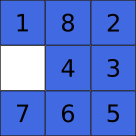
\includegraphics[width=.14\linewidth]{8puzzle-example.pdf}
    \label{fig:8puzzle}
  }\hspace{3em}
  \subfloat[目的の状態]{
    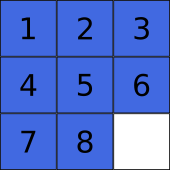
\includegraphics[width=.14\linewidth]{8puzzle-goal.pdf}
    \label{fig:8puzzle-goal}
  }
  \caption{8パズルの状態}
\end{figure}

\begin{algorithm}[H]
  \caption{深さ優先探索}
  \label{algo:depth-first-search}
  \begin{algorithmic}[1]
    \Procedure{DepthFirstSearch}{}
    \State $Stack\gets(初期状態)$
    \While{$|Stack|>0$}
    \State $state\gets pop(Stack)$
    \If{$state$が終了条件を満たす}
    \State \textbf{return} $state$
    \Comment 探索成功
    \EndIf
    \ForAll{$state$に適応可能なオペレータ$operator$}
    \State $push(Stack, operator(state))$
    \Comment オペレータの適応
    \EndFor
    \EndWhile
    \State \textbf{return} $\varnothing$
    \Comment 探索失敗
    \EndProcedure
  \end{algorithmic}
\end{algorithm}

\section{一般化ムーアグラフへの適応}
\label{sect:apply-to-gmg}
本節では,\ref{sect:depth-first-search}節で説明した深さ優先探索を用いて,
一般化ムーアグラフを発見する方法を述べる.探索の初期状態と状態空間に
ついて説明した後,オペレータの適応について説明する.
最後に,これらと定理\ref{thm:gmg-geometric-property}を組み合わせることで
全体的なアルゴリズムを与える.

まず,次のムーアバウンドを定義する.
\begin{definition}
  \textbf{ムーアバウンド}(\textbf{Moore bound})とは,
  次数が$k$,直径が$D$の正則グラフの頂点数の上界で,次式で定義される.
  \begin{equation}
    n_{k,D} = 1 + \sum_{i=1}^Dk(k-1)^{i-1}
  \end{equation}
\end{definition}
これは,同一の次数で$R=0$,$Q=D$の一般化ムーアグラフの頂点数に等しい.
ムーアバウンドを用いて基本となる初期グラフ(\textbf{基本初期グラフ})を定義する.
\begin{definition}[基本初期グラフ]
  \label{def:basic-initial-graph}
  基本初期グラフとは,次のグラフ$G_I$である.
  \begin{equation}
    \begin{aligned}
      \label{eq:basic-initial-graph}
      G_I&=(V,E) \\
      V&=\{1,\ldots,n\} \\
      E&=\{(1,2),\ldots,(1,k+1)\}\cup
      \{(\text{parent}(v),v)|v=k+2,\ldots,n-R\} \\
      \text{parent}(v)&=
      \left\lceil\frac{v-n_{k,\hat{Q}(v)-1}}{k-1}\right\rceil+n_{k,\hat{Q}(v)-2}
    \end{aligned}
  \end{equation}
\end{definition}
基本初期グラフの例を図\ref{fig:initial-tree-example}に示す.

次に,探索空間の基底となる辺の列を定義する.
\begin{definition}[\textbf{候補辺}]
  \label{def:candidate-edges}
  候補辺$\{e_i\}_{i\in\mathbb{N}}$とは,初期グラフ$G_I$に対して,
  $G_I$上で次数が$k$未満の頂点同士を隣接させる辺のうち,$G_I$に属していない
  辺の集合に順序を付加した列である.具体的には,次の式で定義される.
  \begin{equation}
    \{e_i\}_{i\in\mathbb{N}} =
    \{(v,w)\,|\,d_{G_I}(v)<k,d_{G_I}(w)<k,(v,w)\in[V]^2\}\setminus E(G_I)
  \end{equation}
  便宜上,候補辺に属する辺も候補辺と呼ぶことにする.
\end{definition}
候補辺の定義より,一般化ムーアグラフの探索の探索空間は,候補辺から任意の個数の
辺を取り出した組合せと言える.
図\ref{fig:initial-tree-example}に対する候補辺を
図\ref{fig:feasible-edges-example}に破線で示す.

\begin{figure}
  \centering
  \begin{minipage}{.35\columnwidth}
    \def\svgwidth{\textwidth}
    \input{initial-tree-example.pdf_tex}
    \captionof{figure}{頂点数12,次数3の初期グラフ}
    \label{fig:initial-tree-example}
  \end{minipage}
  \hspace{9em}
  \begin{minipage}{.35\columnwidth}
    \def\svgwidth{\textwidth}
    \input{feasible-edges-example.pdf_tex}
    \captionof{figure}{図\ref{fig:initial-tree-example}のグラフに対する候補辺}
    \label{fig:feasible-edges-example}
  \end{minipage}
\end{figure}

探索に用いる状態として,グラフ$G$と次に追加する候補辺の番号$i$の組を使う.
初期状態は,$(G_I,1)$である.状態$(G,i)$が与えられたとき,
候補辺$e_i$を追加するオペレータ(\textbf{追加オペレータ})と
追加しないオペレータ(\textbf{無追加オペレータ})の動作を与える.
追加オペレータは,与えられた状態$(G,i)$に対して,状態$(G+e_i,i+1)$を返す.
また,無追加オペレータは,与えられた状態$(G,i)$に対して,状態$(G,i+1)$を返す.

オペレータが適応可能な条件を示すため,次の記号を定義する.
\begin{definition}
  頂点$v$と候補辺$\{e_i\}_{i\in\mathbb{N}}$について,$v$と接続している辺
  $e_i$の番号$i$の最小値と最大値をそれぞれ$\text{Enter}(v)$と
  $\text{Exit}(v)$とする.
  $\text{Enter}(v)$と$\text{Exit}(v)$の具体的な式は,次で与えられる.
  \begin{equation}
    \label{eq:frontier}
    \begin{aligned}
    \text{Enter}(v) &= \min\{i\,|\,v\in e_i\} \\
    \text{Exit}(v) &= \max\{i\,|\,v\in e_i\}
    \end{aligned}
  \end{equation}
\end{definition}

二種類のオペレータそれぞれについて,対象の辺以降の辺の選び方で
一般化ムーアグラフとなる見込みがあるかどうかを判定する方法を,
定理\ref{thm:gmg-geometric-property}より与える.
\begin{corollary-without-proof}
  \label{coll:basic-add-operator}
  追加オペレータについて,与えられたグラフを$G$,候補辺番号を$i$,候補辺を
  $e_i=\{v,w\}$,適応後のグラフを$G'$とする.$i$以降の候補辺$\{e_j\}_{j>i}$の
  選び方次第で$G'+E\,(E\subset \{e_j\}_{j>i})$が一般化ムーアグラフとなる見込み
  があることは,次の二条件を同時に満たすことである.
  \begin{enumerate}
  \item 次数条件$\cdots$ $d_G(v)<k$かつ,$d_G(w)<k$かつ,
    $\text{Exit}(x)=i$なる$x\in e_i$について$d_{G'}(x)=k$
  \item 閉路条件$\cdots$ $d_G(v,w)\geq2Q$\\
    (この条件を満たすとき,$e_i$によってできる閉路の長さは少なくとも
    $2Q+1$となり,定理\ref{thm:gmg-geometric-property}を満たす)
  \end{enumerate}
\end{corollary-without-proof}
\begin{corollary-without-proof}
  \label{coll:basic-noadd-operator}
  無追加オペレータについて,与えられたグラフを$G$,候補辺番号を$i$,候補辺を
  $e_i=\{v,w\}$,適応後のグラフを$G'=G$とする.$i$以降の候補辺$\{e_j\}_{j>i}$の
  選び方次第で$G'+E\,(E\subset \{e_j\}_{j>i})$が一般化ムーアグラフとなる見込み
  があることは,次の二条件を同時に満たすことである.
  \begin{enumerate}
  \item 次数条件$\cdots$ $\text{Exit}(x)=i$なる$x\in e_i$について,$d_{G'}(x)=k$
  \end{enumerate}
\end{corollary-without-proof}
次は,追加オペレータの適応可能性を判定する例を示している.
\begin{example}
  再び頂点数12,次数3の場合について考える.
  いくつかの辺を追加した後のグラフを図\ref{fig:feasible-edges-example2}に
  示す.図\ref{fig:feasible-edges-example2}に示した辺
  $\{9,10\}$と$\{9,11\}$と$\{9,12\}$について考える.
  辺$\{9,10\}$を追加すると,$d(9,10)=2$のため長さ3の閉路$\{4,\,9,\,10\}$が
  できてしまい,一般化ムーアグラフの条件を満たさなくなる.
  そのため,辺$\{9,10\}$は追加せず次の辺に進む.
  辺$\{9,11\}$についても同様で,長さ4の閉路ができてしまうため,辺を追加しない.
  辺$\{9,12\}$は,$d(9,12)=5$なので長さ6の閉路が複数できる.これは,
  $6>2Q$なので,辺を追加できる.
\end{example}
\begin{figure}
  \centering
  \def\svgwidth{.35\textwidth}
  \input{feasible-edges-example2.pdf_tex}
  \caption{探索途中の状態}
  \label{fig:feasible-edges-example2}
\end{figure}

最後に,説明した事柄を用いて深さ優先探索を一般化ムーアグラフの探索に適応する.
そのアルゴリズムをアルゴリズム\ref{algo:basic-algorithm}に示す.
\begin{algorithm}[H]
  \caption{一般化ムーアグラフの探索アルゴリズム}
  \label{algo:basic-algorithm}
  \begin{algorithmic}[1]
    \Require $n,k$
    \Ensure $M(n,k)\:$(見つからない場合,$\varnothing$を返す)
    \Procedure{FindGeneralizedMooreGraph}{}
    \State $G_I\gets\text{初期グラフ}$
    \Comment 定義\ref{def:basic-initial-graph}
    \State $\{e_i\}_{i\in\mathbb{N}}^M\gets G_I\text{の候補辺}$
    \Comment 定義\ref{def:candidate-edges}
    \State $Stack\gets((G_I,1))$
    \While{$|Stack|>0$}
    \State $G,i\gets pop(Stack)$
    \If{$i>M$かつ
      $G$が正則で定理\ref{thm:gmg-geometric-property}を満たす}
    \State \textbf{return} $G$
    \Comment 探索成功
    \EndIf
    \ForAll{$operator\in\{\text{無追加オペレータ},\text{追加オペレータ}\}$}
    \If{$operator$が$(G,i)$に適応できる}
    \Comment 系\ref{coll:basic-add-operator}と系\ref{coll:basic-noadd-operator}
    \State $push(Stack,operator(G,i))$
    \EndIf
    \EndFor
    \EndWhile
    \State \textbf{return} $\varnothing$
    \Comment 探索失敗
    \EndProcedure
  \end{algorithmic}
\end{algorithm}
アルゴリズム\ref{algo:basic-algorithm}に手を加えて,一般化ムーアグラフを
列挙することができる.
8行目のグラフ返却の前にスタック($Stack$)を保存しておき,
次回以降の呼び出しの4行目で,保存したスタックから再開することで実現する.
列挙の結果に同型なグラフが含まれることに注意する.
アルゴリズム\ref{algo:basic-algorithm}において,6行目が実行される回数を
\textbf{展開状態数}と呼び,高効率化の指標の一つとする.

\section{実験}
\label{sect:exp-basic-algorithm}
本章で提案した方法の性能を測定するための実験を行う.実験で以下の項目を測定する.
\begin{enumerate}
\item 探索開始から最初の一般化ムーアグラフの発見に要する時間
\item 探索開始から最初の一般化ムーアグラフの発見までの展開状態数
\item 一般化ムーアグラフの列挙における,列挙されたグラフ数
\end{enumerate}
実験のパラメータは,次数を$k=3,4$,頂点数を
\begin{equation*}
  \begin{aligned}
    n=\begin{cases}
      4,6,8,10,12,14,16,18 & (k=3) \\
      5,6,7,8,9,10,11,12 & (k=4)
    \end{cases}
  \end{aligned}
\end{equation*}
とする.
本実験での実行環境は表\ref{tab:env-lab}のとおりである.
\begin{table}
  \caption{実行環境}
  \label{tab:env-lab}
  \centering
  \begin{tabular}{ll}
    \hline
    プロセッサ & Intel® Core™ i5-4670 CPU @ 3.40GHz × 4 \\ \hline
    メインメモリ & 5.8GiB \\ \hline
    ベースシステム & Ubuntu 16.04.3 LTS 64 ビット \\ \hline
    仮想化 & Oracle VirtualBox バージョン 5.1.18 r1140024 \\ \hline
    コンパイラ & gcc 5.4.0 \\ \hline
    グラフライブラリ & igraph 0.7.1-2.1 \\ \hline
    最適化フラグ & -Ofast \\ \hline
  \end{tabular}
\end{table}

\section{結果}
\label{sect:result-basic-algorithm}
探索開始から最初の一般化ムーアグラフの発見までに要した探索時間を
図\ref{fig:basic-time}に示す.探索開始から最初の一般化ムーアグラフの発見までの
状態展開数を図\ref{fig:basic-state}に示す.さらに,一般化ムーアグラフの列挙で
取り出されたグラフ数を図\ref{fig:basic-ngraph}に示す.

結果から,すべての測定値について,同一の$Q$の値に対して$R$が大きいほど値が
増加していることが言える.また,$k=3$の結果より,$n=10$を境に指数のベキが
大きくなっている.つまり,$Q$が大きくなるほど指数のベキが大きくなることが
言える.

\begin{figure}
  \centering
  \includegraphics{basic-time-ylab.pdf}
  \includegraphics{basic-time-d3-yaxis.pdf}\hspace{-3mm}
  \subfloat[$k=3$]{
    \includegraphics{basic-time-d3.pdf}
  }\hspace{5mm}
  \includegraphics{basic-time-d4-yaxis.pdf}\hspace{-3mm}
  \subfloat[$k=4$]{
    \includegraphics{basic-time-d4.pdf}
  }
  \includegraphics{basic-time-rpad.pdf}
  \caption{最初の一般化ムーアグラフの発見までの時間}
  \label{fig:basic-time}
\end{figure}

\begin{figure}
  \centering
  \includegraphics{basic-state-ylab.pdf}
  \includegraphics{basic-state-d3-yaxis.pdf}\hspace{-3mm}
  \subfloat[$k=3$]{
    \includegraphics{basic-state-d3.pdf}
  }\hspace{5mm}
  \includegraphics{basic-state-d4-yaxis.pdf}\hspace{-3mm}
  \subfloat[$k=4$]{
    \includegraphics{basic-state-d4.pdf}
  }
  \includegraphics{basic-state-rpad.pdf}
  \caption{最初の一般化ムーアグラフの発見までの展開状態数}
  \label{fig:basic-state}
\end{figure}

\begin{figure}
  \centering
  \includegraphics{basic-ngraph-ylab.pdf}
  \includegraphics{basic-ngraph-d3-yaxis.pdf}\hspace{-3mm}
  \subfloat[$k=3$]{
    \includegraphics{basic-ngraph-d3.pdf}
  }\hspace{5mm}
  \includegraphics{basic-ngraph-d4-yaxis.pdf}\hspace{-3mm}
  \subfloat[$k=4$]{
    \includegraphics{basic-ngraph-d4.pdf}
  }
  \includegraphics{basic-ngraph-rpad.pdf}
  \caption{列挙された一般化ムーアグラフの数}
  \label{fig:basic-ngraph}
\end{figure}
